 
To evaluate interactive smart shelf, we tested it more than once time in real world scenarios. We find some strengths and weakness after the evaluation of our project. Moreover we done seven activities during evaluation that are listed in a below table.

\subsection{Strength} 
\begin{description}
  \item[$\bullet$] The design of drawers are reliable,long lasting and have Multiple User Interface.
   \item[$\bullet$] Color of LED'S follows cultural analogy, i.e. Red (no item), Blue (have an item) and Yellow (<=half amount) in each drawer.
   \item[$\bullet$] If there isn't any item or have less than half amount of an items in drawers, send notification email to administrator.
   \item[$\bullet$] Web application smoothly start service mode that depicts the current state of smart shelf.
   \item[$\bullet$] More than one user can search items simultaneously.
   \item[$\bullet$] Using QR code user can get detail information of items i.e. capacity of resistors etc.
   \end{description}
\subsection{weakness}
\begin{itemize}
  \item Keep small circuit inside each drawer is not good idea.It became messy with items even LED'S inside drawer is not clearly visible for visualization.
  \item Most important keep a plastic plate on the top of load sensor to fix load sensor inside drawer does not give proper measurement.
  \item  Power supply is also an issue, when multiple drawers connect with micro controller.
  \item Place a QR code outside of each small drawer is also a challenge.
\end{itemize}
\subsection{Best Scenarios} 
  The project works best when search any item in drawer and scan QR code to get further detail through web app. Although proper communication is established between web app and micro controller via MQTT protocol. 
\subsection{Failed Scenarios}
 Sometimes when service mode start/stop, LED'S are not properly ON/OFF because of inefficient power supply. Power supply for Arduino is crucial as it stop works at any random point of time in between of service mode which is not good. Further More load sensor does not show accurate weight of items owing to resistance in between plastic plate and drawer.
A broken of MQTT connection immediately would lead to loss of communication between Micro controller and Web app.
\subsection{User Testing} 
We tried web app Smart Shelf with different users and observe while they were doing these activities. These activities are listed in a given table.
%
\begin{figure}
	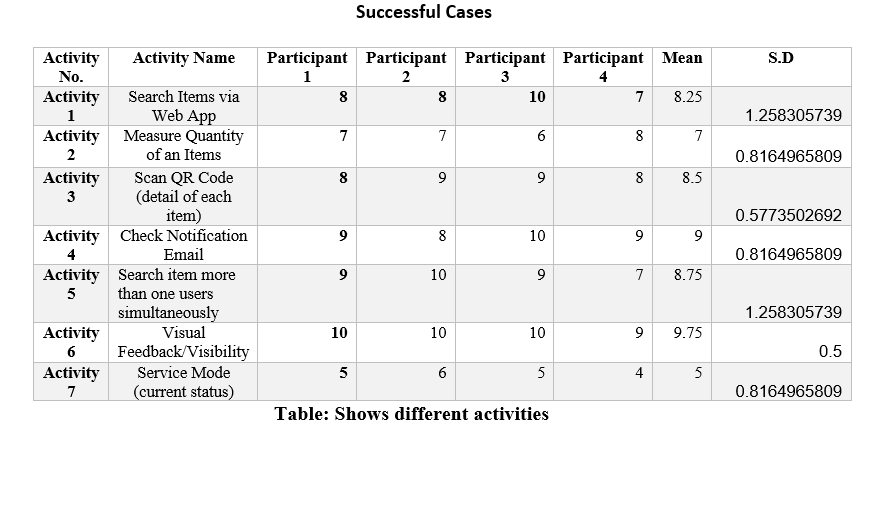
\includegraphics[width=1.1\columnwidth]{figures/table}
	\caption{Table}~\label{fig:table}
\end{figure}
%
\\
We tested all these activities with different 4 participants and get feedback about this web app. The participants were from different age groups range from 22 to 30 years old people some was employee and some were students. For each participant performed each activity 10 times as mention in table. Then we evaluated the number of successful observations, false results and no response. We calculated the percentage of successful observations for each activity and each participant perform these activities and reasons of fault results.

For activity 1 and 5, we found our system is working properly almost 88 percent cases was matched with accepted results according to our observation.
While for activity 2, the system was relatively less accurate as compared to the first activity. more than once time the system does not show perfect. In 70 percent cases the system measured the weight of items correctly but 22 percent the system failed to measure quantity of items. because to calculate quantity was depend on accurate weight measurement but sometimes load sensor interpret wrong weight. That's why with 3rd participant the success rate was 81 percent as compared to the 2nd one. 
Meanwhile activity 6 had high percentage of correct cases with 99 percent among the other all activities.
As we went further and test activity 4 and 5, achieved success ratio over 96 percent, 4 percent cases was failed because of incorrect operations performed by novel users.
In Contrast the last activity, 55 percent cases was failed because of the system was behave unintentionally and inefficient power supply to micro controller was also a critical issue. So the result was not fine among all of above mention activities as 72 percent cases were failed because of inefficient power supply. Participants give bad feedback when they stopped service mode the LED'S was still blinked and system became unresponsive. 
At the end we conclude overall success rate of our smart shelf web app in the light of these 7 activities was 90 percent was perfect as shown in fig (a). As this figure represent the overall evaluation report in form of chart. But 10 percent was unsatisfied owing to some reasons that is mention above.
%
\begin{figure}
	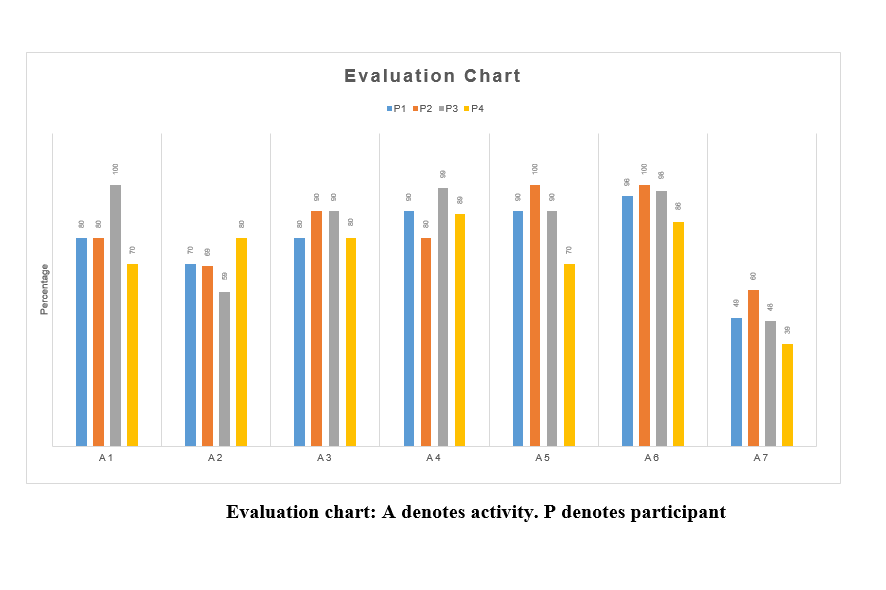
\includegraphics[width=1.1\columnwidth]{figures/Chart}
	\caption{Chart}~\label{fig:Chart}
\end{figure}
%

